\documentclass[tikz,border=2pt]{standalone}
\usepackage{amsmath,amssymb}
\usepackage{tikz}
\usetikzlibrary{arrows.meta}

\begin{document}
% An idempotent matrix (A^2 = A) is a projection: the plane splits into the range (fixed
% pointwise) and the kernel (sent to 0), and applying A twice is the same as once.
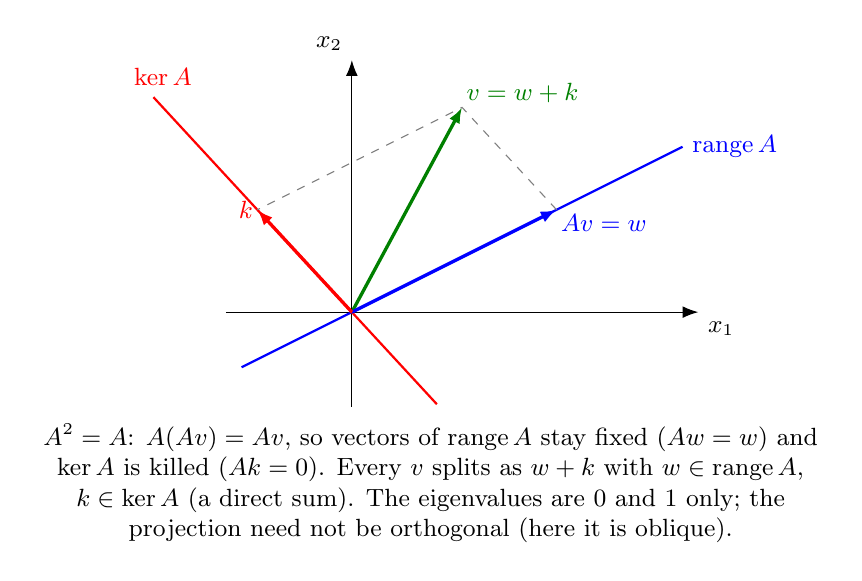
\begin{tikzpicture}[every node/.style={font=\small}, >={Latex[length=2mm]}]
	\draw[->] (-1.6,0) -- (4.4,0) node[below right] {$x_1$};
	\draw[->] (0,-1.2) -- (0,3.2) node[above left] {$x_2$};
	\draw[blue, thick] (-1.4,-0.7) -- (4.2,2.1);
	\node[blue, anchor=west] at (4.2,2.1) {$\operatorname{range}A$};
	\draw[red, thick] (1.08,-1.17) -- (-2.52,2.73);
	\node[red, anchor=south] at (-2.4,2.75) {$\ker A$};
	\draw[->, green!50!black, very thick] (0,0) -- (1.4,2.6) node[above right, inner sep=1pt] {$v=w+k$};
	\draw[->, blue, very thick] (0,0) -- (2.6,1.3) node[below right, inner sep=1pt] {$Av=w$};
	\draw[->, red, very thick] (0,0) -- (-1.2,1.3) node[left, inner sep=1pt] {$k$};
	\draw[dashed, gray] (2.6,1.3) -- (1.4,2.6) -- (-1.2,1.3);
	\node[anchor=north, align=flush center, text width=10cm] at (1.0,-1.3) {$A^2=A$: $A(Av)=Av$, so vectors of $\operatorname{range}A$ stay fixed ($Aw=w$) and $\ker A$ is killed ($Ak=0$). Every $v$ splits as $w+k$ with $w\in\operatorname{range}A$, $k\in\ker A$ (a direct sum). The eigenvalues are $0$ and $1$ only; the projection need not be orthogonal (here it is oblique).};
\end{tikzpicture}
\end{document}
